\chapter{Simulation of on-~and off-shell \ttbar production with \bbfourl}
\label{ch:bb4l}

\section{Introduction}

The accurate modeling of top quark production processes at the LHC is of crucial importance for precision measurement of top quark properties. In particular, the fact the the top quark is an unstable resonance with a short lifetime presents challenges for correctly modeling its mass lineshape as used for top mass and width measurements. \todo{references} Typically, the modeling is done with full NLO MC simulations matched to a parton shower (NLO+PS), and multiple such generators are available with different features and degrees of accuracy.

In this chapter, the predictions of some of these generators from the \powheg framework~\cite{Powheg:2004,Powheg:2007} are compared to each other, as well as to unfolded data measured in \citere{ATLAS:2018ivx}, for different variables relevant to top mass and/or width measurements. A particular focus is the generator \bbfourl \cite{Jezo:2016ujg}, which specifically improves the treatment of the unstable top resonance and of the interference between \ttbar and tW, and is described in detail in \cref{sec:bb4l:bb4l}. The comparison is done using the CMS simulation setup at the generator level, i.e. including parton showering and hadronization but not detector simulation and experimental reconstruction.

The results of this work have been published in a CMS public note as \citere{CMS:NOTE-2023-015}. Since the publication of this note, a new version of \bbfourl has been made available~\cite{Jezo:2023rht}, leading to small differences as discussed below. In this thesis, updated results including both versions will be shown.

\section{The Monte Carlo generator \bbfourl}
\label{sec:bb4l:bb4l}

\bbfourl ~\cite{Jezo:2016ujg,Jezo:2023rht} is a full NLO+PS MC generator for the process $pp \to b \bar{b} \ell^+ \ell^- \nu_\ell \bar{\nu}_\ell$, including all off-shell contributions. This includes the dilepton decay channel of both \ttbar and tW production, as well as non-resonant contributions involving Z or Higgs bosons, as shown in \cref{fig:bb4l:feynman}. Since these processes all lead to the same final state at NLO in QCD, they interfere which each other and can not be easily seperated. \bbfourl includes this interference by construction since it considers the full amplitude including all diagrams at once.

\begin{figure}[h]
    \centering
    \begin{tikzpicture}[baseline=(current bounding box.center)]
      \begin{feynman}
        \vertex (i1) {\(g\)};
        \vertex [below=2.0 cm of i1] (i2) {\(g\)};
        \vertex [right=1.5 cm of i1] (a);
        \vertex [right=1.5 cm of i2] (b);
        \vertex [right=1.0 cm of a] (c);
        \vertex [right=1.0 cm of b] (d);
        \vertex [above right=0.15 cm and 0.75 cm of c] (fb1) {\(b\)};
        \vertex [below right=0.15 cm and 0.75 cm of c] (fW1) {\(W^+\)};
        \vertex [above right=0.15 cm and 0.75 cm of d] (fW2) {\(W^-\)};
        \vertex [below right=0.15 cm and 0.75 cm of d] (fb2) {\(\bar{b}\)};
        \diagram* {
          (i1) -- [gluon] (a),
          (i2) -- [gluon] (b),
          (c) -- [anti fermion, edge label'=\(t\)] (a) -- [anti fermion, edge label'=\(t\)] (b) -- [anti fermion, edge label'=\(\bar{t}\)] (d),
          (c) -- [fermion] (fb1),
          (c) -- [boson] (fW1),
          (d) -- [anti fermion] (fb2),
          (d) -- [boson] (fW2),
        };
      \end{feynman}
    \end{tikzpicture}
    \hfill
    \begin{tikzpicture}[baseline=(current bounding box.center)]
      \begin{feynman}
        \vertex (i1) {\(g\)};
        \vertex [right=1.5 cm of i1] (a);
        \vertex [below=2.0 cm of i1] (i2) {\(g\)};
        \vertex [below=1.25 cm of a] (b);
        \vertex [right=1.0 cm of a] (c);
        \vertex [right=1.0 cm of i2] (d);
        \vertex [above right=0.15 cm and 0.75 cm of c] (fb1) {\(b\)};
        \vertex [below right=0.15 cm and 0.75 cm of c] (fW1) {\(W^+\)};
        \vertex [right=1.75 cm of b] (fW2) {\(W^-\)};
        \vertex [right=2.25 cm of d] (fb2) {\(\bar{b}\)};
        \diagram* {
          (i1) -- [gluon] (a),
          (i2) -- [gluon] (d),
          (c) -- [anti fermion, edge label'=\(t\)] (a) -- [anti fermion, edge label'=\(t\)] (b) -- [anti fermion, edge label'=\(b\)] (d),
          (c) -- [fermion] (fb1),
          (c) -- [boson] (fW1),
          (d) -- [anti fermion] (fb2),
          (b) -- [boson] (fW2),
        };
      \end{feynman}
    \end{tikzpicture}
    \hfill
    \begin{tikzpicture}[baseline=(current bounding box.center)]
      \begin{feynman}
        \vertex (i1) {\(g\)};
        \vertex [below=2.0 cm of i1] (i2) {\(g\)};
        \vertex [right=1.5 cm of i1] (a);
        \vertex [right=1.5 cm of i2] (b);
        \vertex [below=1.0 cm of a] (c);
        \vertex [right=1.0 cm of c] (d);
        \vertex [right=2.0 cm of a] (fb1) {\(b\)};
        \vertex [above right=0.15 cm and 0.75 cm of d] (fW2) {\(W^+\)};
        \vertex [below right=0.15 cm and 0.75 cm of d] (fW1) {\(W^-\)};
        \vertex [right=2.0 cm of b] (fb2) {\(\bar{b}\)};
        \diagram* {
          (i1) -- [gluon] (a),
          (i2) -- [gluon] (b),
          (fb1) -- [anti fermion] (a) -- [anti fermion, edge label'=\(b\)] (c) -- [anti fermion, edge label'=\(b\)] (b) -- [anti fermion] (fb2),
          (c) -- [boson, edge label'=\(Z\mathrm{,}\gamma\)] (d),
          (d) -- [boson] (fW1),
          (d) -- [boson] (fW2),
        };
      \end{feynman}
    \end{tikzpicture}
    \caption{\textbf{Feynman diagrams for \bbfourl.} Examples of Feynman diagrams for the $pp \to b \bar{b} W^+ W^-$ process as described by \bbfourl, including double-resonant (left), single-resonant (center) and non-resonant contributions (right). The decay of the W bosons into leptons is not shown for brevity.}
    \label{fig:bb4l:feynman}
\end{figure}

In addition, by considering the full amplitude instead of splitting it into production and decay parts, \bbfourl fully treats the top quark as an unstable resonance without approximations. It is implemented in the "resonance-aware" version of \powheg, called \powhegvres~\cite{Jezo:2015aia}, which includes hard QCD radiation also in unstable resonances - such as top quarks - in addition to the initial state radiation always provided by \powheg. As a result, an event generated by \bbfourl can have up to three hard emissions already at matrix element level. The correct description of these FSR emissions is relevant e.g. for observables related to the mass of the top quark, and can be challenging for parton showers, leading to large uncertainties.

This work investigates two different versions of \bbfourl. The first version is the one originally published in \citere{Jezo:2016ujg} and publically available on the \powheg website~\cite{Powheg:website}. In the following, it will be referred to as \bbfourl v1.

The second version of \bbfourl was recently published in \citere{Jezo:2023rht}. Its most prominent feature compared to the previous version is the addition of the lepton+jets decay channel of \ttbar, i.e. the $b \bar{b} \ell \nu_{\ell} q \bar{q}'$ final state. In addition, it includes several improvements to the dilepton final state, such as avoidance of spurious finite width effects and improved resonance history projectors (see \citere{Jezo:2023rht} for details). At the time of writing this thesis, the new code is not publically available. A preview version was made available to the CMS collaboration by the authors, and the dilepton final state of this version - referred to as \bbfourl v2 - is shown in this work. The lepton+jets final state, on the other hand, was not ready for validation in the preview version, and so could not be included.

\section{Other \ttbar Monte Carlo generators}
\label{sec:bb4l:others}

The distributions predicted by \bbfourl are compared to three other MC generators for the \tttW final state, which are briefly presented in this section. All of these are implemented in \powhegvtwo, and as such do not contain explicit treatment of radiation in unstable resonances.

\subsection{\hvq}

\hvq~\cite{Frixione:2007nw} is the standard code used, at the time of writing, by both the ATLAS and CMS collaborations for producing \ttbar MC events. It applies the narrow-width approximation (NWA) to generate stable \ttbar pairs at NLO in QCD, with up to one additional ISR emission. The top quarks are then randomly smeared according to the top quark width, giving a rough estimate of finite-width effects. The top quarks are then decayed - here, in the dilepton channel for all lepton flavors - using internal \powheg routines~\cite{Frixione:2007zp}. These routines work at tree level with NLO matrix element corrections and preserve spin correlations. Further ISR emissions as well as all FSR emissions are handled by the matching to the parton shower.

\subsection{\ST}

Since \hvq generates only the double-resonant \ttbar amplitude, a second generator has to be used alongside it for the single-resonant tW and \tttW interference contributions. Here, \ST~\cite{Re:2010bp} is used for this purpose. It works very similar to \hvq, also generating a stable tW pair in the NWA, smearing with the top width and decaying the particles using the same routines.

However, in order to at least approximately recover the full $b \bar{b} W^+ W^-$ amplitude, it is necessary to select a scheme for the treatment of the \tttW interference to prevent double-counting. Since the seperation between \ttbar and tW is not well defined at NLO, such schemes will to some degree always be ad-hoc and ambiguous. Two such schemes are implemented for \ST, and both are compared in this work: In the first, called diagram removal (DR), all terms involving the square of double-resonant diagrams are simply removed from the squared amplitude. This is the most intuitive choice, but has the disadvantage of not being gauge invariant~\cite{Frixione:2008yi}. The second method, diagram subtraction (DS), keeps double-resonant diagrams in the squared amplitude, and subtracts a gauge invariant counter-term to remove the double counting~\cite{Tait:1999cf,Frixione:2008yi,Re:2010bp}. For both schemes, the prediction of \ST is added to the one of \hvq (together called \tttWsum) to produce distributions that can be compared to \bbfourl.

\subsection{\ttb}

The generator \ttb~\cite{Campbell:2014kua}, similar to \hvq, works in the NWA and thus generates stable \ttbar pairs with ad-hoc smearing. However, unlike \hvq, it is fully NLO-accurate not only in the production, but also in the decay of the top quarks. This means that, like \bbfourl, it generates up to one hard FSR emission per decaying top quark, leading to up to three hard emissions in the final state. 

It also provides an LO-accurate treatment of the \tttW interference by reweighting the generated \ttbar events to the full off-shell LO amplitude. Thus, like \bbfourl, it can be used on its own and does not need to be added together with e.g. \ST, but is expected to work at a lower accuracy since it includes more approximations.

\section{Technical setup}

For all generators, LHE events were generated stand-alone and then showered and hadronized with the multi-purpose generator \pythia. Wherever possible, the same settings were used for the different generators, an overview of which can be found in \cref{tab:bb4l:settings}. They are mostly identical to the default settings used by CMS for MC generation, as discussed in \citere{CMS:GEN-17-001}.

\begin{table}
\centering
\begin{tabular}{|cc|}
    \hline
    Parameter & Value \\
    \hline
    \multicolumn{2}{|c|}{\powheg settings} \\
    Top quark mass & \SI{172.5}{\GeV} \\
    Top quark width & \SI{1.33}{\GeV} \\
    \hdamp & $1.38 \, m_t$~\cite{CMS:TOP-16-021} \\
    PDF set & NNPDF 3.1~\cite{NNPDF:2017mvq}\\[.2cm]
    \multicolumn{2}{|c|}{\pythia settings} \\
    \pythia version & 8.307 \\
    \pythia tune & CP5~\cite{CMS:GEN-17-001}\\[.2cm]
    \multicolumn{2}{|c|}{\texttt{PowhegHooks} settings~\cite{Pythia:2022}} \\
    \texttt{POWHEG:veto} & \texttt{on} \\
    \texttt{POWHEG:pThard} & 0 \\
    \texttt{POWHEG:pTdef} & 1 \\
    \hline
\end{tabular}
\caption{\textbf{Generator settings.} An overview of the settings for \powheg and \pythia, as well as the matching between them, for all considered generators.}
\label{tab:bb4l:settings}
\end{table}

\subsection{Parton shower matching}

Special care has to be taken regarding the matching of the \powheg ME generators to the parton shower as provided by \pythia~\cite{Pythia:2022}. In particular, since \powheg already generates events with one or more hard or soft emissions, depending on the process, these configurations must be removed in some form from the \pythia shower to prevent double-counting~\cite{Corke:2010zj}.

In the naive approach, this is achieved by starting the parton shower in \pythia only at the hardness scale of the emission generated by \powheg (sometimes called "wimpy shower"). This way, only additional softer emissions are generated by the shower, and double-counting is avoided. However, this works only as long as the hardness scale definitions in \powheg and \pythia are the same. In practice, they are equal approximately but not exactly, leading to possible inaccuracies.

A more thorough approach can be achieved by always starting the parton shower at the high kinematic limit ("power shower"), calculating the hardness according to the \powheg definition for each generated emission, and vetoing emissions with hardness larger than the emission generated by \powheg. For ISR emissions this method is implemented in \pythia  as part of the \texttt{PowhegHooks} module, and used for all generators considered here.

For \hvq and \ST, which generate only ISR emissions at ME level, this treatment are sufficient. However, for \bbfourl and \ttb, the veto procedure has to be extended to the FSR emissions generated by \powheg in the top decay. This was implemented by the \bbfourl authors in the \texttt{PowhegHooksBB4L} module, a modified form of which is used here, and described in detail in \citere{FerrarioRavasio:2018whr}. Similarly to the ISR case, it is possible to directly start the shower at the hardness scale of the \powheg emission, or employ a veto for emissions above this scale. The latter is used as the default options, and compared to the former in \cref{sec:bb4l:matching}.

\subsection{Same-flavor leptons}
\label{sec:bb4l:sameflavor}

By default, both versions of \bbfourl generate only dilepton final states with opposite-flavor leptons (electrons, muons or $\tau$ leptons). This is because, in principle, there are additional diagrams contributing to the $b \bar{b} \ell^+ \ell^- \nu_\ell \bar{\nu}_\ell$ amplitude for same-flavor leptons, such as $b \bar{b} ZZ$ with $ZZ \rightarrow \ell^+ \ell^- \nu_\ell \bar{\nu}_\ell$, that are not included in \bbfourl.

In practice, the effect of these diagrams will be small, especially in experimental analyses where a cut is applied to reject resonant same-flavor lepton pairs close to the Z boson mass (compare \cref{sec:ttxs:channels}). To make sure that \bbfourl can be used in CMS for experimental analyses involving all lepton flavors, a relabeling procedure already included in \bbfourl is extended to produce also same-flavor lepton final states, neglecting the above mentioned diagrams. This procedure is used for all \bbfourl distributions shown in this chapter.

\section{Results}

\subsection{Comparison between generators}

In this section, the two \bbfourl versions are compared between each other, as well as to the alternative generators introduced in \cref{sec:bb4l:others}, for different observables. All of these comparisons are done after parton showering and hadronization, but without any detector simulation.

The package \rivet~\cite{Rivet:2019rhm} was used to analyze the events. For some observables, publically available analysis packages were employed, which is stated in the captions of the figures where applicable. Furthermore, some observables include distributions at the jet level, which are obtained by running an anti-$k_\mathrm{T}$ algorithm with distance parameter $\Delta R = 0.4$ (AK4)~\cite{Cacciari:2008gp}.

\paragraph{Lepton observables.} To begin the comparison, events with at least two dressed leptons of opposite sign satisfying $\pt > \SI{20}{\GeV}$ and $\abseta < 2.4$ are selected. The \pt distributions of the leading and subleading of these two leptons are shown in \cref{fig:bb4l:leppt}. They show good agreement between the generators within the scale uncertainties, with \tttWsum in the DR scheme predicting a slightly harder lepton spectrum then the others.

\begin{figure}[tp]
    \centering
    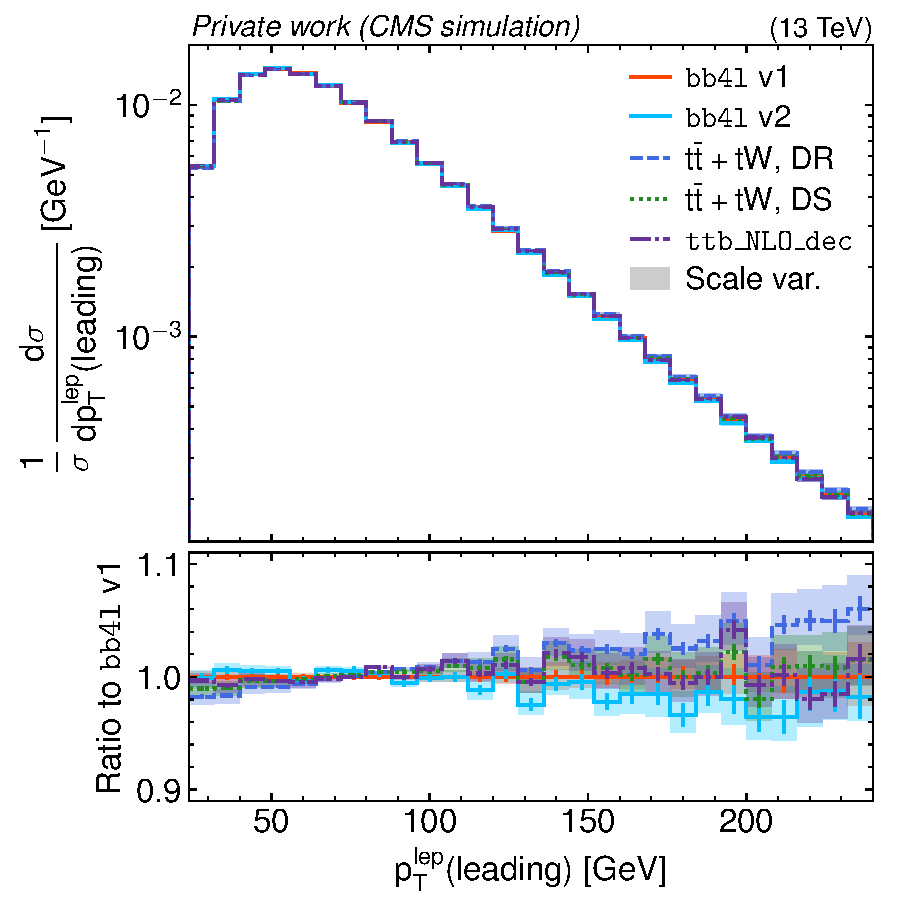
\includegraphics[width=0.49 \textwidth]{figures/bb4l/generators/MC_TTBAR_DILEP_SPINDENSITY_lep_pt_1.pdf}
    \hfill
    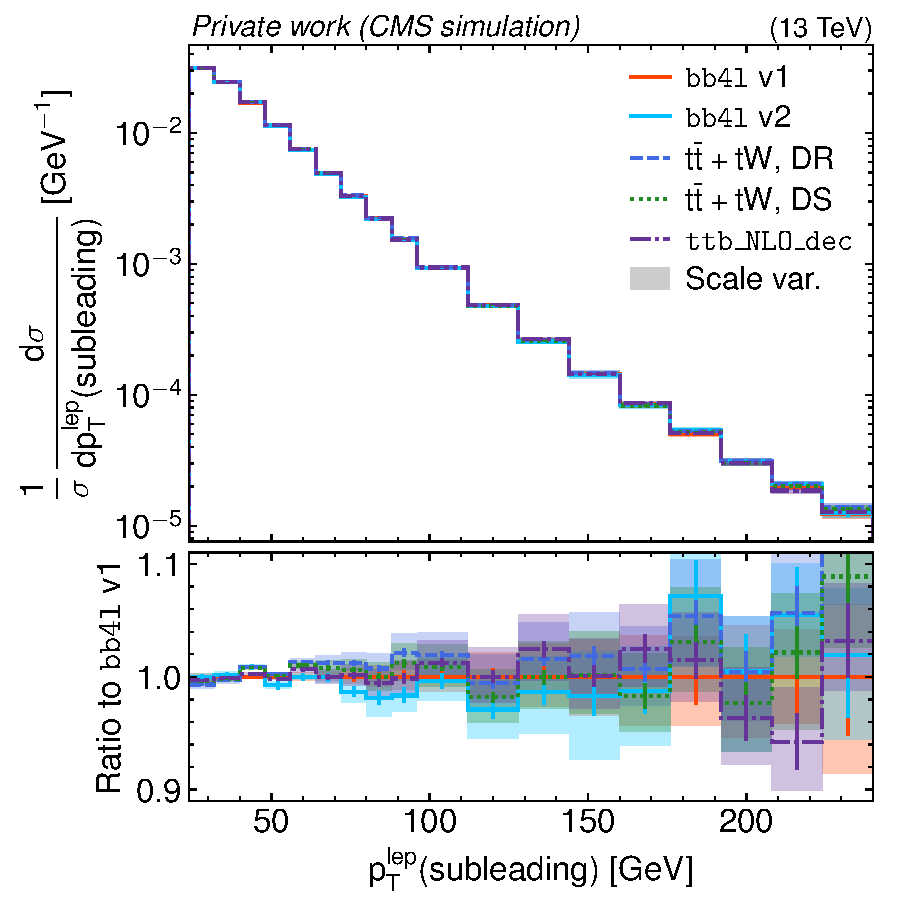
\includegraphics[width=0.49 \textwidth]{figures/bb4l/generators/MC_TTBAR_DILEP_SPINDENSITY_lep_pt_2.pdf}
    \caption{Distributions of the leading (left) and subleading
      (right) lepton \pt for
      \bbfourl v1 (red), v2 (aqua), \tttWsum with the DR (blue) and DS scheme
      (green), as well as \ttb (magenta). The shaded bands show the
      uncertainty due to scale variations, while the error bars show
      the statistical uncertainty.}
    \label{fig:bb4l:leppt}
\end{figure}

The same trend can be seen in \cref{fig:bb4l:mll} for the invariant lepton mass \mll, both inclusively and split by lepton flavor channels. The per-channel distributions are all comparable within statistical uncertainties, which validates the extension to same-flavor leptons for \bbfourl presented in \cref{sec:bb4l:sameflavor}.

\begin{figure}[tp]
    \centering
    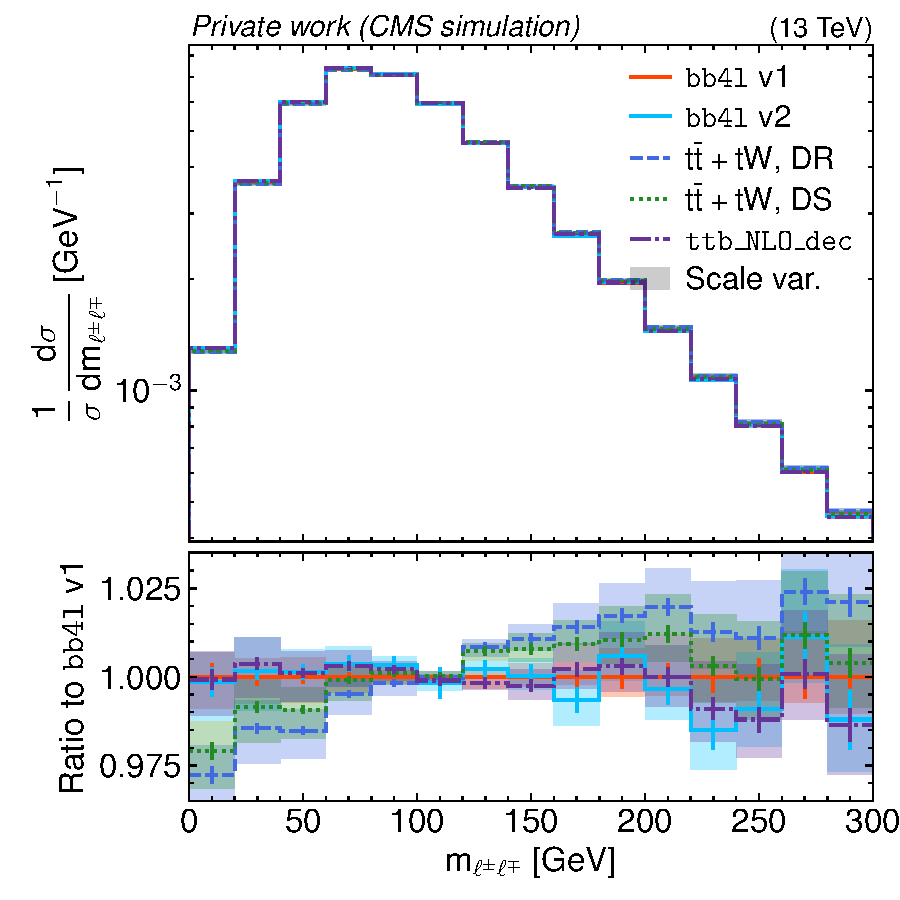
\includegraphics[width=0.49 \textwidth]{figures/bb4l/generators/MC_TTBAR_DILEP_SPINDENSITY_mll.pdf}
    \hfill
    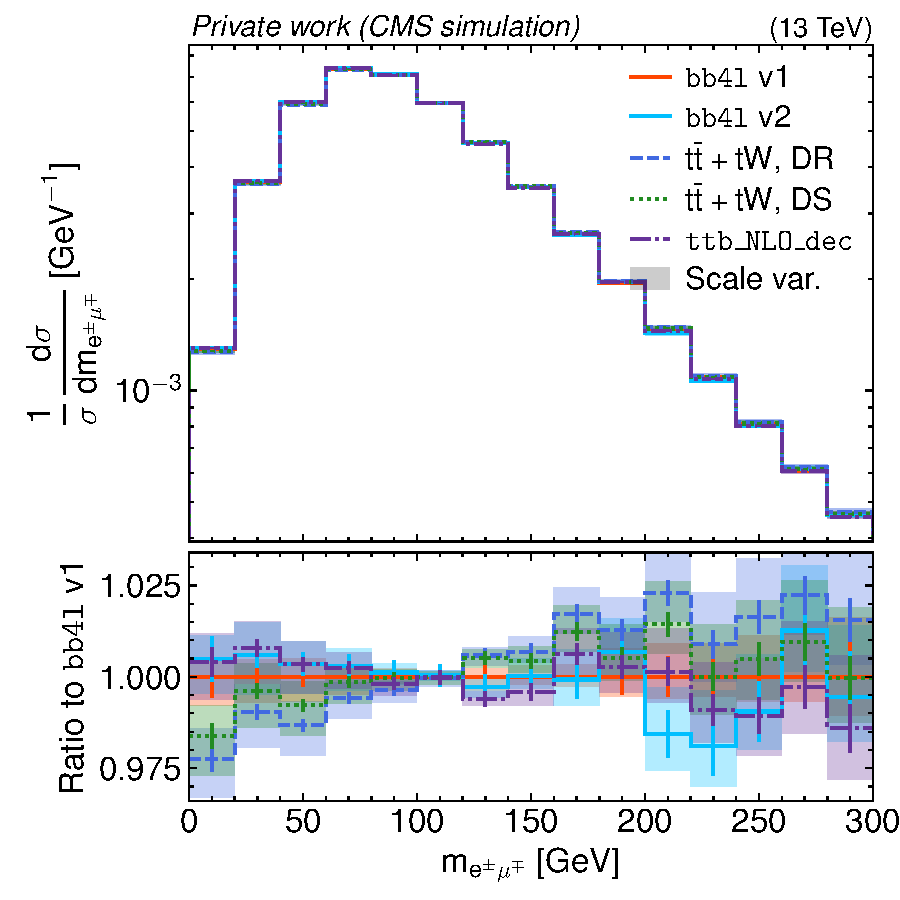
\includegraphics[width=0.49 \textwidth]{figures/bb4l/generators/MC_TTBAR_DILEP_SPINDENSITY_mll_emu.pdf}
    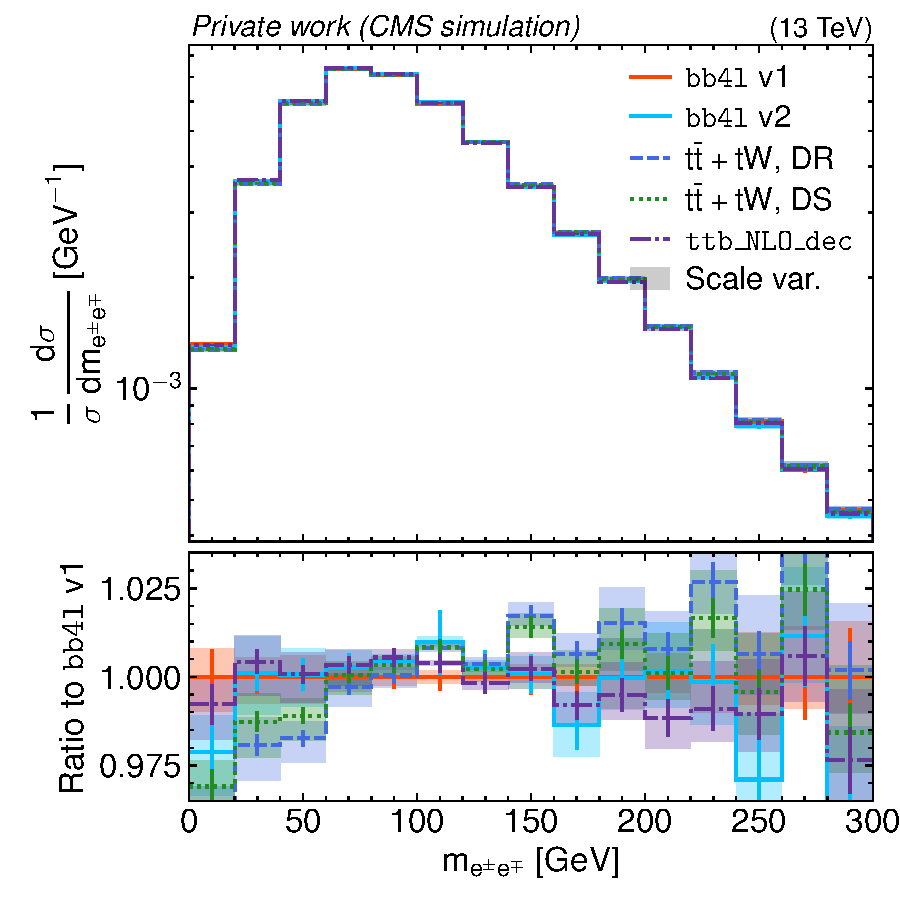
\includegraphics[width=0.49 \textwidth]{figures/bb4l/generators/MC_TTBAR_DILEP_SPINDENSITY_mll_ee.pdf}
    \hfill
    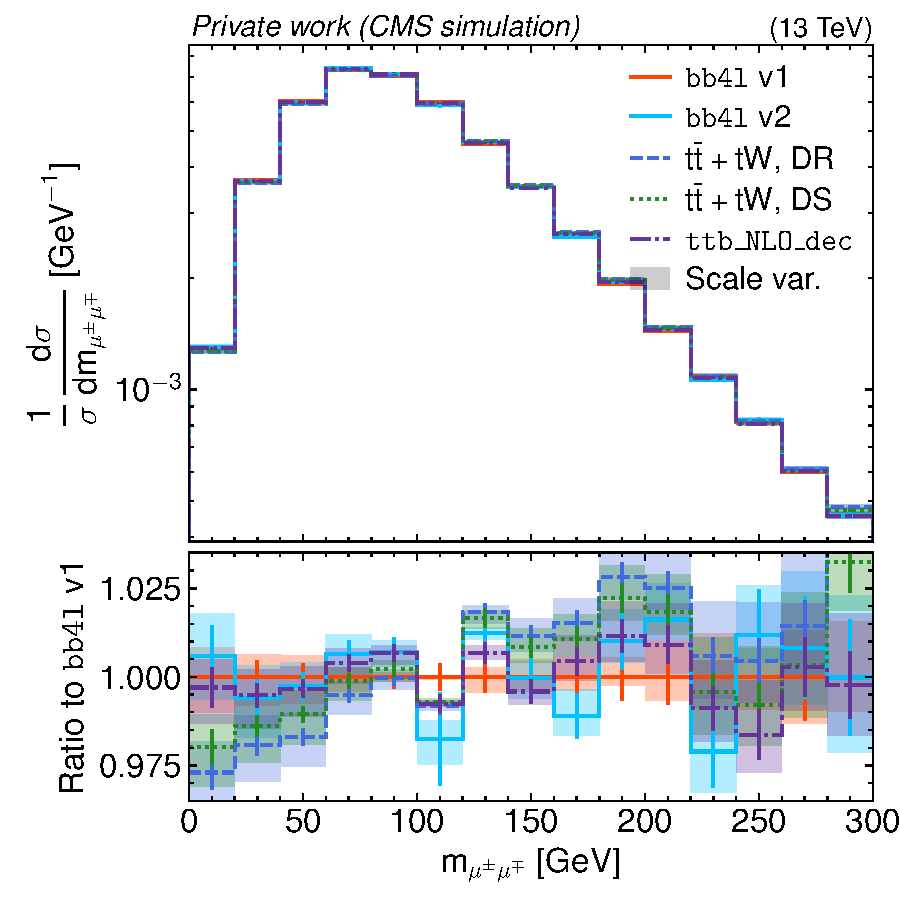
\includegraphics[width=0.49 \textwidth]{figures/bb4l/generators/MC_TTBAR_DILEP_SPINDENSITY_mll_mumu.pdf}
    \caption{Distributions of \mll for all lepton flavors combined (upper left) as well as in the \emu (upper right), \ee (lower left) and \mumu channels (lower right), shown in the same manner as in \cref{fig:bb4l:leppt}.}
    \label{fig:bb4l:mll}
\end{figure}

\paragraph{Jet observables.} 

\subsection{Comparison of FSR matching settings}
\label{sec:bb4l:matching}

\subsection{Recoil in top decay}

\section{Summary}
